%%%%%%%% Klassen-Optionen
\documentclass[12pt,a4paper]{scrartcl}

%%%%%%%% PAKETE: unverzichtbare Pakete mit Einstellungen
\usepackage[left=2.5cm, right=2cm, top=3cm, bottom=3cm, a4paper]{geometry} %Seitenrände
\usepackage[utf8x]{inputenc} % utf8-Kodierung und direkte Eingabe von Sonderzeichen
\usepackage{fixltx2e} % Verbessert einige Kernkompetenzen von LaTeX2e

%%%%%%%% PAKETE: AMS-Pakete
\usepackage{amsmath} % Mathe-Erweiterung
\usepackage{amsfonts} % Schrift-Erweiterung
\usepackage{amssymb} % Sonderzeichen-Erweiterung

%%%%%%%% PAKETE: Sonstiges
\usepackage[colorlinks, citecolor=black, filecolor=black, linkcolor=black, urlcolor=black]{hyperref} % Links
\usepackage{wrapfig} % ausgeklügekte Floatumgebung
\usepackage{float} % normale Floatumgebung
\restylefloat{figure} % ermöglicht die Verwendung von "H" (ist noch stärker als "h!")
\usepackage[small,it,singlelinecheck=false]{caption} % Bildunterschriften formatieren
\usepackage{multirow} % ermöglich Verbinden von Tabellenzeilen
\usepackage{multicol} % ermöglicht Spalten
\usepackage{fancyhdr} % ermöglicht Kopf- und Fußzeilen
\usepackage{graphicx} % Einbinden von Bildern möglich
\usepackage{units} % Einheiten
\usepackage{subcaption}

%%%%%%%% DEFINITIONEN: Titelseite
\author{April Cooper, Patrick Kreissl und Sebastian Weber}
\title{Worksheet 4: All-atom Molecular Dynamics simulations
of the alanine dipeptide}
\publishers{University of Stuttgart}
\date{\today}

%%%%%%%% ANPASSUNGEN: Kopf-und Fußzeile
\fancypagestyle{plain}{} % redefine the plain pagestyle to match the fancy layout
\pagestyle{fancy} % aktiviere eigenen Seitenstil
\fancyhf{} % alle Kopf- und Fußzeilen bereinigen
\fancyhead[L]{Worksheet 4: All-atom MD simulations
of the alanine dipeptide}
\fancyhead[R]{\today}
\renewcommand{\headrulewidth}{0.6pt} % obere Trennlinie
\fancyfoot[L]{April Cooper, Patrick Kreissl und Sebastian Weber}
\fancyfoot[R]{Page \thepage}
\renewcommand{\footrulewidth}{0.6pt} % untere Trennlinie

%%%%%%%% ANPASSUNGEN: Absätze
\setlength{\parindent}{0em} % keine Absatzeinzüge
\setlength{\parskip}{0.5em} % Absatz-Abstand

%%%%%%%% ANPASSUNGEN: Abbildungsverzeichnis
\usepackage{tocloft} % Zum Anpassen der Verzeichnisse
%\renewcommand{\cftfigpresnum}{Abb. }
%\renewcommand{\cfttabpresnum}{Tab. }
\renewcommand{\cftfigaftersnum}{:}
\renewcommand{\cfttabaftersnum}{:}
\setlength{\cftfignumwidth}{2cm}
\setlength{\cfttabnumwidth}{2cm}
\setlength{\cftfigindent}{0cm}
\setlength{\cfttabindent}{0cm}

%%%%%%%% SONSTIGES
\usepackage{pdfpages}
\usepackage{pgf}
%\usepackage{subfigure}
\usepackage{graphicx}
\usepackage{caption}
\usepackage{subcaption}


% NÜTZLICH: http://truben.no/latex/table/

% Anfang des eigentlichen Dokuments
\begin{document}

\maketitle
\tableofcontents
\newpage

\section{Performing the energy minimization}
After converting the alanine dipeptides *.pdb file into a *.gro file, adding a simulation box around the protein, filling it up with water and preprocessing the simulation by using a proper *.mdp file, the energy minimization run can be started. Energy minimization makes sure that a certain maximum force (given by the *.mdp file) is not exceeded by any of the operating bonding forces in the simulation. Very large forces mean a great amount of potential energy stored which would be released during the real simulation. This would result in a enormous increase of the time required for equilibration.

The -v option of mdrun makes the program verbose. Therefore it prints out the maximum bond width, potential energy, maximum force plus the involved atom for each simulation step. This is done until the maximum force converged to Fmax(simulation) $<$ Fmax(mdp file). The result is a *.gro file of the energy minimized structure.

\section{Performing the warm up and the simulation}
Using the energy minimized structure and another *.mdp file a warmup simulation is preprocessed and performed. The entries in the used *.mdp file tell among others what integrator to use (here used: md means leap frog integrator), which time to simulate, which simulation time step to use, the thermostat type (here: berendsen thermostat), and the desired temperature (here: 300 K).

After that, these entries are modified and the simulation is preprocessed using the new *.mdp file and the warmed up simulation state as starting state for the real simulation. Then the real simulation can be run.

\section{Calculating the distribution of the dihedral angles}
The distribution of the dihedral angles is visualized by a ramachandran plot (figure \ref{fig:ala}). It visualizes the dihedral angles $\varphi$ and $\psi$. The positioning of most measuring points at negative $\varphi$ and slightly negative $\psi$ generally indicate $\alpha$-helices as secondary structure elements. $\beta$-sheets are indicated by positioning at positive $\psi$ and negative $\varphi$. Therefore the ramachandran plot of the simulated alanine dipeptide indicate that the presence of alanine in proteins highly facilitate the building of $\alpha$-helices and is also favourable for building  $\beta$-sheets. 

\begin{figure}[H]
	\centering
	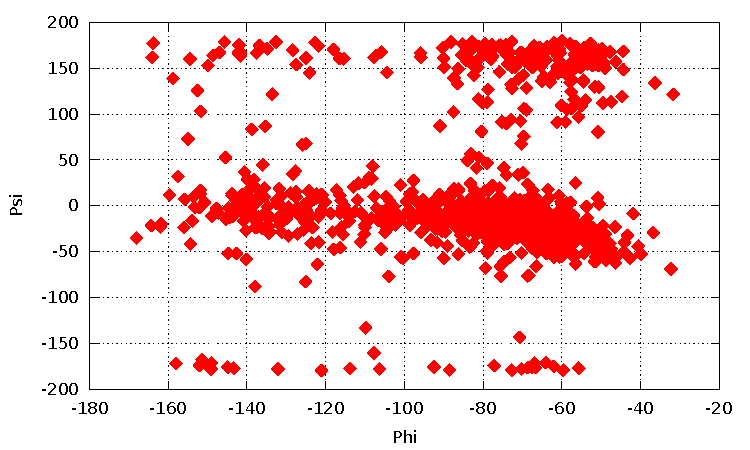
\includegraphics{./plt/rama.pdf}
	\caption{Ramachandran plot of alanine dipeptide}\label{fig:ala}
\end{figure}


\end{document}


% =============== Comments ============
\begin{comment}
\verb{x_init {}}

\begin{figure}[H]
	\resizebox{1\textwidth}{!{\input{../plt/GGA_mesh.pdf}}
	\caption{CAPTION}\label{fig:NAME}
\end{figure}
\end{comment}
